\chapter{应用层}

\begin{quote}
    \centering
    网络应用是计算机网络存在的理由
\end{quote}

\section{应用层协议原理}

    \emph{研发网络应用程序的核心是写出能够运行在不同的端系统和通过网络彼此通信的程序。}

    当研发新应用程序时,你需要编写将在多台端系统上运行的软件。重要的是,你不需要写在网络核心设备如路由器或链路层交换机上运行的软件。即使你要为网络核心设备写应用程序软件,你也不能做到这一点。网络核心设备并不在应用层上起作用,而仅在较低层起作用,特别是在网络层及下面层次起作用。这种基本设计,即将应用软件限制在端系统的方法,促进了大量的网络应用程序的迅速研发和部署。

\subsection{网络应用程序体系结构}

    当进行软件编码之前,应当对应用程序有一个宽泛的体系结构计划。从应用程序研发者的角度看,网络体系结构是固定的,并为应用程序提供了特定的服务集合。在另一方面,应用程序体系结构(application architecture)由应用程序研发者设计, 规定了如何在各种端系统上组织该应用程序。

\subsubsection{客户-服务器体系结构}

    在客户-服务器体系结构(client-server architecture)中,有一个总是打开的主机称为服务器,它服务于来自许多其他称为客户的主机的请求。\emph{值得注意的是利用客户-服务器体系结构,客户相互之间不直接通信}。

    客户-服务器体系结构的另一个特征是该服务器具有固定的、周知的地址,该地址称为IP地址。因为该服务器具有固定的、周知的地址,并且因为该服务器总是打开的,客户总是能够通过向该服务器的IP地 址发送分组来与其联系。

    在一个客户-服务器应用中,常常会出现一台单独的服务器主机跟不上它所有客户请求的情况。为此,配备大量主机的数据中心(data center)常被用于创建强大的虚拟服务器。

\subsubsection{P2P体系结构}

    在一个 P2P 体系结构(P2P architecture)中,对位于数据中心的专用服务器有最小的(或者没有)依赖。相反,应用程序在间断连接的主机对之间使用直接通信,这些主机对被称为对等方。因为这种对等方通信不必通过专门的服务器,该体系结构被称为对等方到对等方的。

    许多目前流行的、流量密集型应用都是P2P体系结构的。需要提及的是,某些应用具有混合的体系结构,它结合了客户-服务器和P2P的元素。

    P2P体系结构的最引人入胜的特性之一是它们的自扩展性(self-scalability)。例如, 在一个P2P文件共享应用中,尽管每个对等方都由于请求文件产生工作负载,但每个对等方通过向其他对等方分发文件也为系统增加服务能力。

\subsection{进程通信}

    用操作系统的术语来说,进行通信的实际上是进程(process)而不是程序。一个进程可以被认为是运行在端系统中的一个程序。当多个进程运行在相同的端系统上时,它们使用进程间通信机制相互通信。进程间通信的规则由端系统上的操作系统确定。

    此处,我们并不特别关注同一台主机上的进程间的通信,而关注运行在不同端系统(可能具有不同的操作系统)上的进程间的通信。

    在两个不同端系统上的进程,通过跨越计算机网络交换报文(message)而相互通信。发送进程生成并向网络中发送报文;接收进程接收这些报文并可能通过回送报文进行响应。

\subsubsection{客户和服务器进程}

    网络应用程序由成对的进程组成,这些进程通过网络相互发送报文。对每对通信进程, 我们通常将这两个进程之一标识为客户(client),而另一个进程标识为服务器(serve)。

    \emph{在一对进程之间的通信会话场景中,发起通信(即在该会话开始时发起与其他进程的联系)的进程被标识为客户,在会话开始时等待联系的进程是服务器}。

\subsubsection{进程与计算机网络之间的接口}

    多数应用程序是由通信进程对组成,每对中的两个进程互相发送报文。进程通过一个称为套接字(sock-et)的软件接口向网络发送报文和从网络接收报文。

    下图显示了两个经过因特网通信的进程之间的套接字通信(图中假定由该进程使用的下面运输层协议是因特网的TCP协议)。如该图所示,套接字是同一台主机内应用层与运输层之间的接口。由于该套接字是建立网络应用程序的可编程接口,因此套接字也称为应用程序和网络之间的应用程序编程接口(Application Programming Interface, API)。应用程序开发者可以控制套接字在应用层端的一切,但是对该套接字的运输层端几乎没有控制权。

\begin{figure}[!htbp]
    \centering
    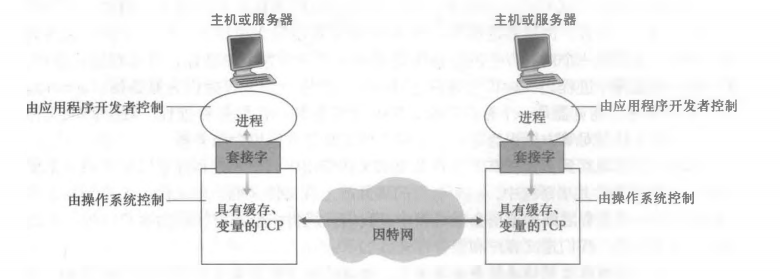
\includegraphics[width=0.6\textwidth]{image/chapter02/应用进程通信.png}
    \caption{应用程序间的套接字通信}
\end{figure}

    应用程序开发者对于运输层的控制仅限于:①选择运输层协议;②也许能设定几个运输层参数,如最大缓存和最大报文段长度等。

\subsubsection{进程寻址}

    在因特网中,主机由其IP地址(IP address)标识。此时,我们只要知道IP地址是一个32比特的量且它能够唯一地标识该主机就够了。除了知道报文发送目的地的主机地址外,发送进程还必须指定运行在接收主机上的接收进程(更具体地说,接收套接字)。因为一般而言一台主机能够运行许多网络应用, 这些信息是需要的。目的地端口号(port number)用于这个目的。

\subsection{可供应用程序使用的运输服务}

    包括因特网在内的很多网络提供了不止一种运输层协议。当开发一个应用时,必须选择一种可用的运输层协议。如何做出这种选择呢?最可能的方式是,通过研究这些可用的运输层协议所提供的服务,选择一个最能为你的应用需求提供恰当服务的协议。

    我们大体能够从四个方面对应用程序服务要求进行分类:可靠数据传输、吞吐量、定时和安全性。

\subsubsection{可靠数据传输}

    分组在计算机网络中可能丢失。在一些应用中,数据丢失可能会造成灾难性的后果。

    因此,为了支持这些应用,必须做一些工作以确保由应用程序的一端发送的数据正确、完全地交付给该应用程序的另一端。如果一个协议提供了这样的确保数据交付服务,就认为提供了可靠数据传输(reliable data transfer)。

    运输层协议能够潜在地向应用程序提供的一个重要服务是进程到进程的可靠数据传输。当一个运输协议提供这种服务时,发送进程只要将其数据传递进套接字,就可以完全相信该数据将能无差错地到达接收进程。

\subsubsection{吞吐量}

    在沿着一条网络路径上的两个进程之间的通信会话场景中,可用吞吐量就是发送进程能够向接收进程交付比特的速率。

    运输层协议能够以某种特定的速率提供确保的可用吞吐量。使用这种服务,该应用程序能够请求r比特/秒的确保吞吐量,并且该运输协议能够确保可用吞吐量总是为至少r比特/秒。这样的确保吞吐量的服务将对许多 应用程序有吸引力。

    具有吞吐量要求的应用程序被称为带宽敏感的应用(bandwidth-sensitive application)。带宽敏感的应用具有特定的吞吐量要求,而弹性应用(elastic application)能够根据当时可用的带宽或多或少地利用可供使用的吞吐量。

\subsubsection{定时}

    运输层协议也能提供定时保证。如同具有吞吐量保证那样,定时保证能够以多种形式实现。一个保证的例子如:发送方注入进套接字中的每个比特到达接收方的套接字不迟于100ms。

\subsubsection{安全性}
    
    运输协议能够为应用程序提供一种或多种安全性服务。这种服务将在发送和接收进程之间提供机密性,以防该数据以某种方式在这两个进程之间被观察到。运输协议还能提供除了机密性以外的其他安全性服务,包括数据完整性和端点鉴别。

\subsection{因特网提供的运输服务}

    我们已经考虑了计算机网络能够提供的通用运输服务。现在我们要更为具体地考察由因特网提供的运输服务类型。因特网(更一般的是TCP/IP网络)为应用程序提供两个运输层协议,即UDP和TCP。

\subsubsection{TCP服务}

    TCP服务模型包括面向连接服务和可靠数据传输服务。当某个应用程序调用TCP作为其运输协议时,该应用程序就能获得来自TCP的这两种服务。

\begin{table*}[!htbp]
    \begin{center}
        \caption{选择的网络应用的要求}
        \begin{tabular}{ | c | c | c | c | }
            \hline
            \textbf{应用} & \textbf{数据丢失} & \textbf{带宽} & \textbf{时间敏感} \\
            \hline
            文件传输 & 不能丢失 & 弹性 & 不 \\
            \hline
            电子邮件 & 不能丢失 & 弹性 & 不 \\
            \hline
            Web文档 & 不能丢失 & 弹性(几 kbps) & 不 \\
            \hline
            \multicolumn{1}{| c |}{\multirow{2}{*}{因特网电话/视频会议}} & \multicolumn{1}{c |}{\multirow{2}{*}{容忍丢失}} & 音频(几 kbps~1 Mbps) & \multicolumn{1}{c |}{\multirow{2}{*}{是,100ms}} \\
            \cline{3-3}
            \multicolumn{1}{| c |}{} & \multicolumn{1}{c |}{} & 视频(10 kbps~5 Mbps) & \multicolumn{1}{c |}{} \\
            \hline
            流式存储音频/视频 & 容忍丢失 & 同上 & 是,几秒 \\
            \hline
            交互式游戏 & 容忍丢失 & 几 kbps~10 kbps & 是,100ms \\
            \hline
            只能手机讯息 & 不能丢失 & 弹性 & 是和不是 \\
            \hline
        \end{tabular}
    \end{center}    
\end{table*}

\begin{itemize}
    \item [1)] 面向连接的服务
    \subitem 在应用层数据报文开始流动之前,TCP让客户和服务器互相交换运输层控制信息。这个所谓的握手过程提醒客户和服务器,让它们为大量分组 的到来做好准备。在握手阶段后,一个TCP连接(TCP connection)就在两个进程的套接字之间建立了。这条连接是全双工的,即连接双方的进程可以在此连接上同时进行报文收发。当应用程序结束报文发送时,必须拆除该连接。
    \item [2)] 可靠的数据传送服务
    \subitem 通信进程能够依靠TCP,无差错、按适当顺序交付所有发送的数据。当应用程序的一端将字节流传进套接字时,它能够依靠TCP将相同的 字节流交付给接收方的套接字,而没有字节的丢失和冗余。
    \item [3)] 拥塞控制机制
    \subitem 这种服务不一定能为通信进程带来直接好处,但能为 因特网带来整体好处。当发送方和接收方之间的网络出现拥塞时,TCP的拥塞控制机制会抑制发送进程(客户或服务器)。
\end{itemize}

\subsubsection{UDP服务}

    UDP是一种不提供不必要服务的轻量级运输协议,它仅提供最小服务。UDP是无连接的,因此在两个进程通信前没有握手过程。UDP协议提供一种不可靠数据传送服务,也就是说,当进程将一个报文发送进UDP套接字时,UDP协议并不保证该报文将到达接收进程。不仅如此,到达接收进程的报文也可能是乱序到达的

    UDP没有包括拥塞控制机制,所以UDP的发送端可以用它选定的任何速率向其下层(网络层)注入数据。(然而,值得注意的是实际端到端吞吐量可能小于该速率,这可能是因为中间链路的带宽受限或因为拥塞而造成的。)

\subsubsection{因特网运输协议所不提供的服务}

    在我们对TCP和UDP的简要描述中,明显地漏掉了对吞吐量或定时保证的讨论,即这些服务目前的因特网运输协议并没有提供。

    下表指出了一些流行的因特网应用所使用的运输协议。

\begin{table*}[!htbp]
    \begin{center}
        \caption{流行的因特网应用及其应用层协议与支撑的运输协议}
        \begin{tabular}{| c | c | c |}
            \hline
            \textbf{应用} & \textbf{应用层协议} & \textbf{支撑的运输协议} \\
            \hline
            电子邮件 & SMTP[ RFC 5321 ] & TCP \\
            \hline
            远程终端访问 & Telnet[ RFC 854 ] & TCP \\
            \hline
            Web & HTTP[ RFC 2616 ] & TCP \\
            \hline
            文件传输 & FTP[ RFC 959 ] & TCP \\
            \hline
            流式多媒体 & HTTP(如YouTube) & TCP \\
            \hline
            因特网电话 & SIP[ RFC 3261 ]、RTP[ RFC 3550 ] 或专用的(如Skype) & UDP或TCP \\
            \hline
        \end{tabular}
    \end{center}
\end{table*}

\subsection{应用层协议}

    应用层协议(application-layer protocol)定义了运行在不同端系统上的应用程序进程如何相互传递报文。特别是应用层协议定义了:

\begin{itemize}
    \item [1)] 交换的报文类型,例如请求报文和响应报文
    \item [2)] 各种报文类型的语法,如报文中的各个字段及这些字段是如何描述的
    \item [3)] 字段的语义,即这些字段中的信息的含义
    \item [4)] 确定一个进程何时以及如何发送报文,对报文进行响应的规则
\end{itemize}

    区分网络应用和应用层协议是很重要的。应用层协议只是网络应用的一部分(尽管从我们的角度看,它是应用非常重要的一部分)。

\section{Web和HTTP}

    Web是一个引起公众注意的因特网应用,它极大地改变了人们与工作环境内外交流的方式。它将因特网从只是很多数据网之一的地位提升为仅有的一个数据网。

\subsection{HTTP概况}

    Web的应用层协议是超文本传输协议(HyperText Transfer Protocol, HTTP),它是Web的核心。HTTP由两个程序实现:一个客户程序和一个服务器程序。客户程序和服务器程序运行在不同的端系统中,通过交换HTTP报文进行会话。HTTP定义了这些报文的结构以及客户和服务器进行报文交换的方式。

    Web页面(Webpage)(也叫文档)是由对象组成的。一个对象(object)只是一个文件,诸如一个HTML文件、一个JPEG图形、一个Java小程序或一个视频片段这样的文件,且它们可通过一个URL地址寻址。多数Web页面含有一个HTML基本文件(base HTML file)以及几个引用对象。

    HTML基本文件通过对象 的URL地址引用页面中的其他对象。每个URL地址由两部分组成:存放对象的服务器主机名和对象的路径名。Web服务器(Webserver)实现了HTTP的服务器端,它用于存储Web对象,每个对象由URL寻址。

    HTTP定义了Web客户向Web服务器请求Web页面的方式,以及服务器向客户传送Web页面的方式。如下图所示,客户与服务器交互的过程。

\begin{figure}[!htbp]
    \centering
    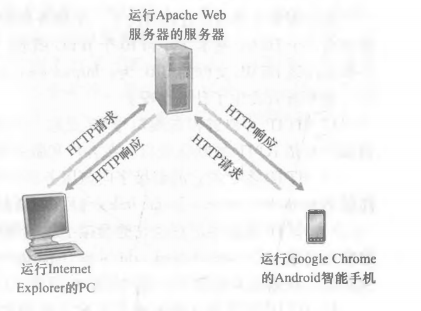
\includegraphics[width=0.6\textwidth]{image/chapter02/HTTP服务.png}
    \caption{HTTP请求-响应行为}
\end{figure}

    HTTP使用TCP作为它的支撑运输协议(而不是在UDP上运行)。HTTP客户首先发起一个与服务器的TCP连接。一旦连接建立,该浏览器和服务器进程就可以通过套接字接口访问TCP。

    客户向它的套接字接口发送HTTP请求报文并从它的套接字接口接收HTTP响应报文。类似地,服务器从它的套接字接口接收HTTP请求报文和向它的套接字接口发送HTTP响应报文。一旦客户向它的套接字接口发送了一个请求报文,该报文就脱离了客户控制并进入TCP的控制。

    这里我们看到了分层体系结构最大的优点,即\emph{HTTP协议不用担心数据丢失,也不关注TCP从网络的数据丢失和乱序故障中恢复的细节。那是TCP以及协议栈较低层协议的工作}。

    \emph{服务器向客户发送被请求的文件,而不存储任何关于该客户的状态信息。假如某个特定的客户在短短的几秒内两次请求同一个对象,服务器并不会因为刚刚为该客户提供了该对象就不再做出反应,而是重新发送该对象,就像服务器已经完 全忘记不久之前所做过的事一样。因为HTTP服务器并不保存关于客户的任何信息},所以我们说HTTP是一个无状态协议(stateless protocol)。

\subsection{非持续连接和持续连接}

    在许多因特网应用程序中,客户和服务器在一个相当长的时间范围内通信,其中客户发出一系列请求并且服务器对每个请求进行响应。依据应用程序以及该应用程序的使用方 式,这一系列请求可以以规则的间隔周期性地或者间断性地一个接一个发出。当这种客 户-服务器的交互是经TCP进行的。

    应用程序的研制者就需要做一个重要决定,即每个请求/响应对是经一个单独的TCP连接发送,还是所有的请求及其响应经相同的TCP连接发送呢?采用前一种方法,该应用程序被称为使用非持续连接(non-persistent connection);采用后一种方法,该应用程序被称为使用持续连接(persistent connection)。

\subsubsection{采用非持续连接的HTTP}

    我们看看在非持续连接情况下,从服务器向客户传送一个Web页面的步骤。假设该页面含有一个HTML基本文件和10个JPEG图形,并且这11个对象位于同一台服务器上。进 一步假设该 HTML 文件的 URL 为:http :〃www. someSchool. edu/someDepartment/home, indexo 我们看看发生了什么情况: 
    
\begin{itemize}
    \item [1)] HTTP客户进程在端口号80发起一个到服务器www.someSchool.edu的TCP连接,该端口号是HTTP的默认端口。在客户和服务器上分别有一个套接字与该连接相关联。
    \item [2)] HTTP客户经它的套接字向该服务器发送一个HTTP请求报文。请求报文中包含了路径名/someDepartment/home.index (后面我们会详细讨论HTTP报文)。 
    \item [3)] HTTP服务器进程经它的套接字接收该请求报文,从其存储器(RAM或磁盘)中 检索出对象 www.someSchool.edu/someDepartment/home.index,在一个 HTTP 响应报文中封装对象,并通过其套接字向客户发送响应报文。
    \item [4)] HTTP服务器进程通知TCP断开该TCP连接。(但是直到TCP确认客户已经完整地收到响应报文为止,它才会实际中断连接。)
    \item [5)] HTTP客户接收响应报文,TCP连接关闭。该报文指岀封装的对象是一个HTML文件,客户从响应报文中提取出该文件,检査该HTML文件,得到对10个JPEG图形的引用
    \item [6)] 对每个引用的JPEG图形对象重复前4个步骤
\end{itemize}

    上面的步骤举例说明了非持续连接的使用,其中每个TCP连接在服务器发送一个对象后关闭,即该连接并不为其他的对象而持续下来。值得注意的是每个TCP连接只传输一个请求报文和一个响应报文。因此在本例中,当用户请求该Web页面时,要产生11个TCP连接。

    我们给出往返时间(Round Trip Time, RTF)的定义,该时间是指一个短分组从客户到服务器然后再返回客户所花费的时间。RTT包括分组传播时延、分组在中间路由器和交换机上的排队时延以及分组处理时延。

\begin{figure}[!htbp]
    \centering
    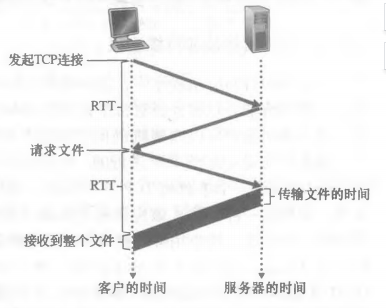
\includegraphics[width=0.6\textwidth]{image/chapter02/RTT.png}
    \caption{请求并接收一个HTML文件所需的时间估算}
\end{figure}

\subsubsection{采用持续连接的HTTP}

    非持续连接有一些缺点:
    
    第一,必须为每一个请求的对象建立和维护一个全新的连接。对于每个这样的连接,在客户和服务器中都要分配TCP的缓冲区和保持TCP变量,这给Web服务器带来了严重的负担,因为一台Web服务器可能同时服务于数以百计不同的客户的请求。

    第二,就像我们刚描述的那样,每一个对象经受两倍RTT的交付时延,即一个RTT用于创建TCP,另一个RTT用于请求和接收一个对象。

    在采用HTTP 1.1持续连接的情况下,服务器在发送响应后保持该TCP连接打开。在相同的客户与服务器之间,后续的请求和响应报文能够通过相同的连接进行传送。一般来说,如果一条连接经过一定时间间隔(一个可配置的超时间隔)仍未被使用,HTTP服务器就关闭该连接。HTTP的默认模式是使用带流水线的持续连接。

\subsection{HTTP报文格式}

HTTP 规范[ RFC 1945; RFC 2616; RFC 7540 ]包含了对HTTP报文格式的定义。HTTP报文有两种:请求报文和响应报文。

\subsubsection{HTTP请求报文}

\begin{lstlisting}[language=C++]
GET /somedir/page.html HTTP/1.1
Host: www.someschool.edu
Connection: close
User-agent: Mozilla/5.0
Accept-language: fr
\end{lstlisting}

    观察这个简单的请求报文,其中有五行信息,\emph{每一行的结尾都有一个结束符号(操作系统不同所对应的结束符号不同,在这里以$'\backslash{r}\backslash{n}'$为准)}。

    HTTP请求报文的第一行叫做请求行(request line),其后继的行叫做首部行(header line)。请求行有3个字段:方法字段、URL字段和HTTP版本字段。

    方法字段可以取几种不同的值,包括GET、POST、HEAD、PUT和DELETEO绝大部分的HTTP请求报文使用GET方法。当浏览器请求一个对象时,使用GET方法,在URL字段带有请求对象的标识。

    现在我们看看本例的首部行。首部行Host:www.someschool.edu指明了对象所在的主机。该首部行提供的信息是Web代理高速缓存所要求的。

    通过包含Connection: close首部行,该浏览器告诉服务器不要麻烦地使用持续连接,它要求服务器在发送完被请求的对象后就关闭这条连接。
    
    User-agent:首部行用来指明用户代理,即向服务器发送请求的浏览器的类型。这里浏览器类型是Mozilla/5.0,即Firefox浏览器。 这个首部行是有用的,因为服务器可以有效地为不同类型的用户代理实际发送相同对象的不同版本。(每个版本都由相同的URL寻址。)
    
    最后,Accept-language:首部行表示用户想得到该对象的法语版本(如果服务器中有这样的对象的话);否则,服务器应当发送它的默认版本。Accept-language:首部行仅是HTTP中可用的众多内容协商首部之一。

    接下来我们来看看请求报文的通用格式:

\begin{figure}[!htbp]
    \centering
    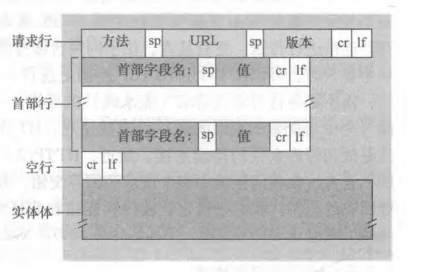
\includegraphics[width=0.6\textwidth]{image/chapter02/请求报文通用格式.png}
    \caption{HTTP请求报文的通用格式}
\end{figure}

    我们发现,在空行后有一个“实体体” (entity body)。\emph{使用GET方法时实体体为空,而使用POST方法时才使用该实体体}。当用户提交表单时,HTTP客户常常使用POST方法。如果方法字段的值为POST时, 则实体体中包含的就是用户在表单字段中的输入值。

    当然,值得注意的是,HTML表单经常使用GET方法,并在(表单字段中)所请求的URL中包括输入的数据。例如,一个表单使用GET方法,它有两个字段,分别填写的是"monkeys"和"bananas",这样,该URL结构为www.somesite.com/animalsearch?monkeys\&bananas。

    HEAD方法类似于GET方法。当服务器收到一个使用HEAD方法的请求时,将会用一个HTTP报文进行响应,但是并不返回请求对象。应用程序开发者常用HEAD方法进行调试跟踪。PUT方法常与Web发行工具联合使用,它允许用户上传对象到指定的Web服务器上指定的路径(目录)。PUT方法也被那些需要向Web服务器上传对象的应用程序使用。DELETE方法允许用户或者应用程序删除Web服务器上的对象。

\subsubsection{HTTP响应报文}

    下面我们提供了一条典型的HTTP响应报文。

\begin{lstlisting}[language=C++]
HTTP/1.1 200 OK
Connection: close
Date: Tue, 18 Aug 2015 15:44:04 GMT
Server: Apache/2.2.3 (CentOS)
Last-Modified: Tuer 18 Aug 2015 15:11:03 GMT
Content-Length: 6821
Content-Type: text/html
(data data data data data ...)
\end{lstlisting}

    我们仔细看一下这个响应报文。它有三个部分:一个初始状态行(status line), 6个首部行(headerline),然后是实体体(entity body)。实体体部分是报文的主要部分,即它包含了所请求的对象本身(表示为data data data data data...)。状态行有3个字段:协议版本字段、状态码和相应状态信息。

    我们现在来看看首部行。
    
    服务器用Connection: close首部行告诉客户,发送完报文后将关闭该TCP连接。
    
    Date:首部行指示服务器产生并发送该响应报文的日期和时间。值得一提的是,这个时间不是指对象创建或者最后修改的时间,而是服务器从它的文件系统中 检索到该对象,将该对象插入响应报文,并发送该响应报文的时间。
    
    Server:首部行指示该报文是由一台ApacheWeb服务器产生的,它类似于HTTP请求报文中的User-agent:首部行。

    Last-Modified:首部行指示了对象创建或者最后修改的日期和时间。Last- Modified:首部行对既可能在本地客户也可能在网络缓存服务器上的对象缓存来说非常重要。我们将很快详细地讨论缓存服务器(也叫代理服务器)。
    
    Content Length: 首部行指示了被发送对象中的字节数。
    
    Content-Type:首部行指示了实体体中的对象是HTML文本。(该对象类型应该正式地由Content-Type:首部行而不是用文件扩展名来指示。)

    接下来我们看一下响应报文的通用格式

\begin{figure}[!htbp]
    \centering
    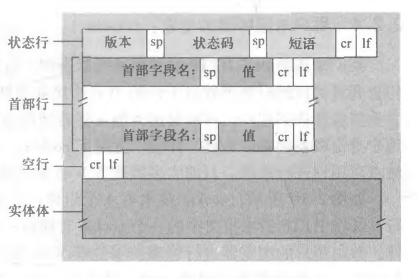
\includegraphics[width=0.6\textwidth]{image/chapter02/响应报文通用格式.png}
    \caption{HTTP响应报文的通用格式}
\end{figure}

    我们补充说明一下状态码和它们对应的短语。状态码及其相应的短语指示了请求的结果。一些常见的状态码和相关的短语包括:

\begin{itemize}
    \item [1)] 200 OK:请求成功,信息在返回的响应报文中
    \item [2)] 301 Moved Permanently:请求的对象已经被永久转移了,新的URL定义在响应报文的Location:首部行中。客户软件将自动获取新的URL
    \item [3)] 400 Bad Request: 一个通用差错代码,指示该请求不能被服务器理解
    \item [4)] 404 Not Found:被请求的文档不在服务器上
    \item [5)] 505 HTTP Version Not Supported:服务器不支持请求报文使用的HTTP协议版本
\end{itemize}

\subsection{用户与服务器的交互:cookie}

    我们前面提到了HTTP服务器是无状态的。这简化了服务器的设计,并且允许工程师们去开发可以同时处理数以千计的TCP连接的高性能Web服务器。

    然而一个Web站点通常希望能够识别用户,可能是因为服务器希望限制用户的访问,或者因为它希望把内容与用户身份联系起来。为此,HTTP使用了 cookie。cookie在[RFC 6265 ]中定义,它允许站点对用户进行跟踪。目前大多数商务Web站点都使用了cookie。

    cookie技术有4个组件:①在HTTP响应报文中的一个cookie首部行;②在HTTP请求报文中的一个cookie首部行;③在用户端系统中保留有一个cookie文 件,并由用户的浏览器进行管理;④位于Web站点的一个后端数据库。

    假设我们在以前访问过一个网站站点,那么在第一次建立连接的时候,该Web站点会产生一个唯一的cookie标识码以此来作为索引在后端数据库中产生一个表项,在后续访问该网站时,首部的响应报文就会包含:

\begin{lstlisting}[language=C++]
Set-cookie: 1678
\end{lstlisting}

    因此,当浏览器收到了该HTTP响应报文,就会将之前用户所注册的信息活动反馈过来。

\begin{figure}[!htbp]
    \centering
    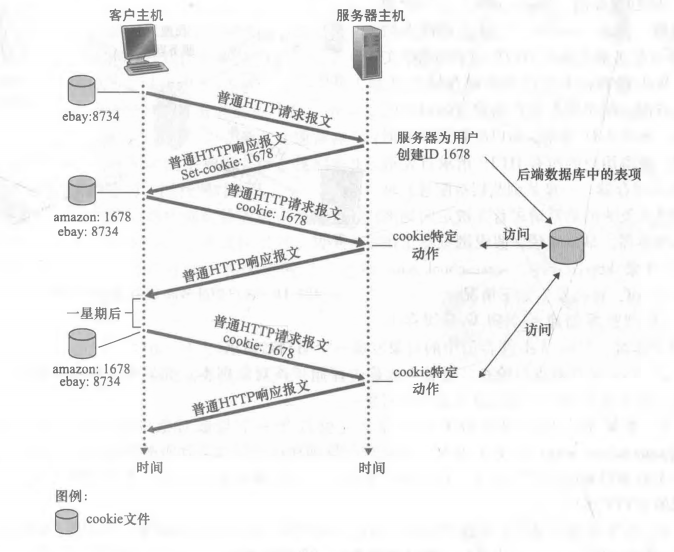
\includegraphics[width=0.6\textwidth]{image/chapter02/cookie.png}
    \caption{用cookie跟踪用户状态}
\end{figure}

\subsection{Web缓存}

    Web缓存器(Web cache)也叫代理服务器(proxy server),它是能够代表初始Web服务器来满足HTTP请求的网络实体。Web缓存器有自己的磁盘存储空间,并在存储空间中保存最近请求过的对象的副本。

\begin{figure}[!htbp]
    \centering
    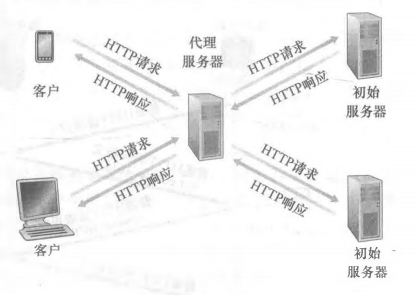
\includegraphics[width=0.6\textwidth]{image/chapter02/Web缓存技术.png}
    \caption{客户通过Web缓存器请求对象}
\end{figure}

    可以配置用户的浏览器,使得用户的所有HTTP请求首先指向Web缓存器。一旦某浏览器被配置,每个对某对象的浏览器请求首先被定向到该Web缓存器。举例来说,假设浏览器正在请求对象http://www.someschool.edu/campus.gif,将会发生如下情况:

\begin{itemize}
    \item [1)] 浏览器创建一个到Web缓存器的TCP连接,并向Web缓存器中的对象发送一个HTTP请求。
    \item [2)] Web缓存器进行检查,看看本地是否存储了该对象副本。如果有,Web缓存器就向客户浏览器用HTTP响应报文返回该对象。
    \item [3)] 如果Web缓存器中没有该对象,它就打开一个与该对象的初始服务器(即WWW. someschool. edu)的TCP连接。Web缓存器则在这个缓存器到服务器的TCP连接上发送一个对该对象的HTTP请求。在收到该请求后,初始服务器向该Web缓存器发送具有该对象的HTTP响应
    \item [4)] 当Web缓存器接收到该对象时,它在本地存储空间存储一份副本,并向客户的浏览器用HTTP响应报文发送该副本(通过现有的客户浏览器和Web缓存器之间的TCP连接)
\end{itemize}

    在因特网上部署Web缓存器有两个原因。首先,Web缓存器可以大大减少对客户请求的响应时间,特别是当客户与初始服务器之间的瓶颈带宽远低于客户与Web缓存器之间的瓶颈带宽时更是如此。其次,Web缓存器能够大大减少一个机构的接入链路到因特网的通信量。

\subsection{条件GET方法}

    尽管高速缓存能减少用户感受到的响应时间,但也引入了一个新的问题,即存放在缓存器中的对象副本可能是陈旧的。

    幸运的是,HTTP协议有一种机制,允许缓存器证实它的对象是最新的。这种机制就是条件GET(conditional GET)方法。如果:①请求报文使用GET方法;并且②请求报文中包含一个“ If Modified-Since: ”首部行。那么,这个HTTP请求报文就是一个条件GET请求报文。

    为了演示,我们给出以下的例子:

    首先,一个代理缓存器(proxy cache)代表一个请求浏览器,向某Web服务器发送一个请求报文:

\begin{lstlisting}[language=C++]
GET /fruit/kiwi.gif HTTP/1.1
Host: www.exotiquecuisine.com
\end{lstlisting}

    其次,该Web服务器向缓存器发送具有被请求的对象的响应报文:

\begin{lstlisting}[language=C++]
HTTP/1.1 200 OK
Date: Sat, 3 Oct 2015 15:39:29
Server: Apache/1.3.0 (Unix)
Last-Modified: Wed, 9 Sep 2015 09:23:24
Content-Type: image/gif
(data data data data data ...)
\end{lstlisting}

    该缓存器在将对象转发到请求的浏览器的同时,也在本地缓存了该对象。重要的是, 缓存器在存储该对象时也存储了最后修改日期。由于在过去的一个星期中位于Web服务器上的该对象可能已经被修改了,该缓存器通过发送一个条件GET执行最新检查。具体来说,该缓存器发送:

\begin{lstlisting}[language=C++]
GET /fruit/kiwi.gif HTTP/1.1
Host: www.exotiquecuisine.com
If-modified-since: Wed, 9 Sep 2015 09:23:24
\end{lstlisting}

    该条件GET报文告诉服务器,仅当自指定日期之后该对象被修改过,才发送该对象。假设该对象自2015年9月9H09:23:24后没有被修改。接下来的第四步,Web服务器向该缓存器发送一个响应报文:

\begin{lstlisting}[language=C++]
HTTP/1.1 304 Not Modified
Date: Satf 10 Oct 2015 15:39:29
Server: Apache/1 3 0 (Unix)
(empty entity body)
\end{lstlisting}

    我们看到,作为对该条件GET方法的响应,该Web服务器仍发送一个响应报文,但并没有在该响应报文中包含所请求的对象。包含该对象只会浪费带宽,并增加用户感受到的响应时间,特别是如果该对象很大的时候更是如此。值得注意的是在最后的响应报文中,状态行中为304 Not Modified,它告诉缓存器可以使用该对象,能向请求的浏览器转发它(该代理缓存器)缓存的该对象副本。

\section{因特网中的电子邮件}

    与普通邮件一样,电子邮件是一种异步通信媒介,即当人们方便时就可以收发邮件,不必与他人的计划进行协调。与普通邮件相比,电子邮件更为快速并且易于分发,而且价格便宜。现代电子邮件具有许多强大的特性,包括具有附件、超链接、HTML格式文本和图片的报文。

    下图展示了了因特网电子邮件系统的总体情况。从该图中我们可以看到它有3个主要组成部分:用户代理(user agent)、邮件服务器(mail server)和简单邮件传输协议(Simple Mail Transfer Protocol, SMTP)。

\begin{figure}[!htbp]
    \centering
    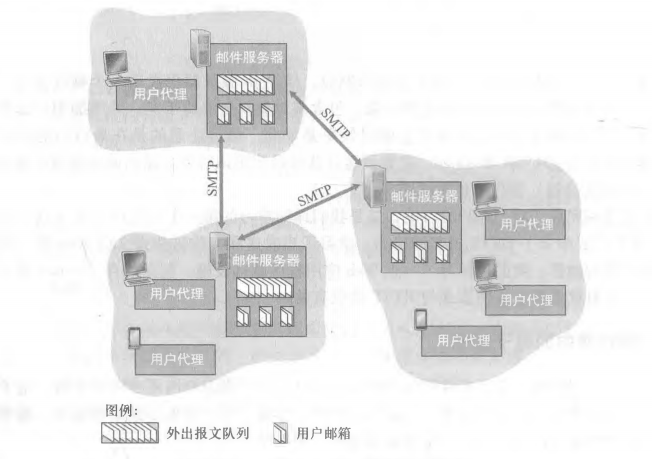
\includegraphics[width=0.6\textwidth]{image/chapter02/电子邮件系统的总体描述.png}
    \caption{电子邮件系统的总体描述}
\end{figure}

    邮件服务器形成了电子邮件体系结构的核心。每个接收方在其中的某个邮件服务器上有一个邮箱(mailbox)。

    一个典型的邮件发送过程是:从发送方的用户代理开始,传输到发送方的邮件服务器,再传输到接收方的邮件服务器,然后在这里被分发到接收方的邮箱中。

    如果发送方的服务器不能将邮件交付给接收方的服务器,发送方的邮件服务器在一个报文队列(message queue)中保持该报文并在以后尝试再次发送。通常每30分钟左右进行一次尝试;如果几天后仍不能成功,服务器就删除该报文并以电子邮件的形式通知发送方。

    SMTP是因特网电子邮件中主要的应用层协议。它使用TCP可靠数据传输服务,从发送方的邮件服务器向接收方的邮件服务器发送邮件。像大多数应用层协议一样,SMTP也有两个部分:运行在发送方邮件服务器的客户端和运行在接收方邮件服务器的服务器端。每台邮件服务器上既运行SMTP的客户端也运行SMTP的服务器端。当一个邮件服务器向其他邮件服务器发送邮件时,它就表现为SMTP的客户;当邮件服务器从其他邮件服务器上接收邮件时,它就表现为一个SMTP的服务器。

\subsection{SMTP}

    SMTP是因特网电子邮件的核心。如前所述,SMTP用于从发送方的邮件服务器发送报文到接收方的邮件服务器。SMTP问世的时间比HTTP要长得多。尽管电子邮件应用在因特网上的独特地位可以证明SMTP有着众多非常岀色的性质,但它所具有的某种陈旧特征表明它仍然是一种继承的技术。

    在SMTP协议中,限制了所有邮件报文的体部分(不只是其首部)只能采用简单的7比特ASCII表示。为了描述SMTP的基本操作,我们来模拟一种场景。假设Alice想给Bob发送一封简单的ASCII报文。

\begin{itemize}
    \item [1)] Alice调用她的邮件代理程序并提供Bob的邮件地址(例如bob@someschool.edu),撰写报文,然后指示用户代理发送该报文
    \item [2)] Alice的用户代理把报文发给她的邮件服务器,在那里该报文被放在报文队列中
    \item [3)] 运行在Alice的邮件服务器上的SMTP客户端发现了报文队列中的这个报文,它就创建一个到运行在Bob的邮件服务器上的SMTP服务器的TCP连接
    \item [4)] 在经过一些初始SMTP握手后,SMTP客户通过该TCP连接发送Alice的报文
    \item [5)] 在Bob的邮件服务器上,SMTP的服务器端接收该报文。Bob的邮件服务器然后将该报文放入Bob的邮箱中
    \item [6)] 在Bob方便的时候,他调用用户代理阅读该报文
\end{itemize}

\begin{figure}[!htbp]
    \centering
    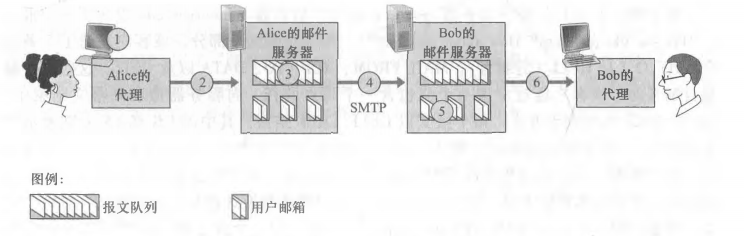
\includegraphics[width=0.6\textwidth]{image/chapter02/SMTP流程.png}
    \caption{一个简单的SMTP邮件传输流程}
\end{figure}

    需要注意的是:\emph{SMTP 一般不使用中间邮件服务器发送邮件,即使这两个邮件服务器位于地球的两端也是这样。假设Alice的邮件服务器在中国香港,而Bob的服务器在美国圣路易斯,那么这个TCP连接也是从香港服务器到圣路易斯服务器之间的直接相连。特别是,如果Bob的邮件服务器没有开机,该报文会保留在Alice的邮件服务器上并等待进行新的尝试,这意味着邮件并不在中间的某个邮件服务器存留}。

    接下来我们分析一个SMTP客户(C)和SMTP服务器(S)之间的交换报文文本的例子,客户的主机名为crepes.fr,服务器的主机名为hamburger.du

\begin{lstlisting}[language=C++]
S: 220 hamburger.edu
C: HELO crepes.fr
S: 250 Hello crepes.fr, pleased to meet you
C: MAIL FROM: <alice@crepes.fr>
S: 250 alice@crepes.fr ... Sender ok
C: RCPT TO: <bob@hamburger.edu>
S: 250 bob@hamburger.edu ... Recipient ok
C: DATA
S: 354 Enter mail, end with "." on a line by itself
C: Do you like ketchup?
C: How about pickles? 
C: .
S: 250 Message accepted for delivery
C: QUIT
S: 221 hamburger.edu closing connection
\end{lstlisting}

    第一行,表示服务器已经准备好与客户端建立连接,第二行则是客户端对服务器表面自己的身份。该客户发送了5条命令:HELO (是 HELLO 的缩写)、MAIL FROM、RCPTTO、DATA以及QUIT。这些命令都是自解释的。该客户通过发送一个只包含一个句点的行,向服务器指示该报文结束了。 (按照ASCII码的表示方法,每个报文以CRLF.CRLF结束,其中的CR和LF分别表示回车和换行。)服务器对每条命令做出回答,其中每个回答含有一个回答码和一些(可选的)英文解释

\subsection{与HTTP的对比}

    这两个协议都用于从一台主机向另一台主机传送文件:HTTP从Web服务器向Web客户(通常是一个浏览器)传送文件(也称为对象);SMTP从一个邮件服务器向另一个邮件服务器传送文件(即电子邮件报文)。

    当然的,两者也有一些重要的区别:

\begin{itemize}
    \item [1)] HTTP主要是一个拉协议(pull protocol),即在方便的时候,某些人在Web服务器上装载信息,用户使用HTTP从该服务器拉取这些信息。特别是TCP连接是由想接收文件的机器发起的。另一方面,SMTP基本上是一个推协议(push protocol),即发送邮件服务器把文件推向接收邮件服务器。特别是,这个TCP连接是由要发送该文件的机器发起的
    \item [2)] SMTP要求每个报文(包括它们的体)采用7比特ASCII码格式。如果某报文包含了非7比特ASCII字符(如具有重音的法文字符)或二进制数据(如图形文件),则该报文必须按照7比特ASCII码进行编码。HTTP数据则不受这种限制
    \item [3)] 是如何处理一个既包含文本又包含图形(也可能是其他媒体类型)的文档。HTTP把每个对象封装到它自己的HTTP响应报文中,而SMTP则把所有报文对象放在一个报文之中。
\end{itemize}

\subsection{邮件报文格式}

    首部行和该报文的体用空行(即回车换行)进行分隔。RFC 5322定义了邮件首部行和它们的语义解释的精确格式。如同HTTP协议, 每个首部行包含了可读的文本,是由关键词后跟冒号及其值组成的。某些关键词是必需的,另一些则是可选的。每个首部必须含有一个From:首部行和一个To:首部行;一个首部也许包含一个Subject:首部行以及其他可选的首部行。重要的是注意到下列事实:这 些首部行不同于我们在之前所学到的SMTP命令(即使那里包含了某些相同的词汇, 如from和to)。那节中的命令是SMTP握手协议的一部分;本节中考察的首部行则是邮件报文自身的一部分。

    一个典型的报文首部看起来如下:

\begin{lstlisting}[language=C++]
From: alice@crepes fr
To: bob@hamburger.edu
Subject: Searching for the meaning of life.
\end{lstlisting}

    在报文首部之后,紧接着一个空白行,然后是以ACSII格式表示的报文体。你应当用Telnet向邮件服务器发送包含一些首部行的报文,包括Subject:首部行

\subsection{邮件访问协议}

    一旦SMTP将邮件报文从Alice的邮件服务器交付给Bob的邮件服务器,该报文就被放入了Bob的邮箱中。在今天,邮件访问使用了一种客户-服务器体系结构,即典型的用户通过在用户端系统上运行的客户程序来阅读电子邮件。

    如果接收方在本地PC上运行用户代理软件库,那么在他的本地PC上放置一个邮件服务器也是自然而然的事情。但是,为了能够及时接收收可能在任何时候到达的新邮件,他的PC必须总是不间断地运行着并一直保持在线。这对于许多因特网用户而言是不现实的。

    现在我们来看以下通信流程:

\begin{figure}[!htbp]
    \centering
    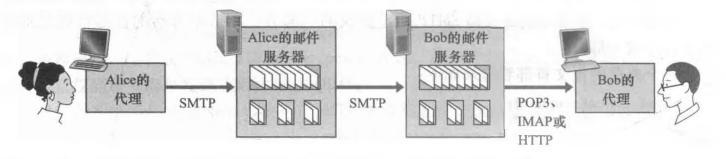
\includegraphics[width=0.6\textwidth]{image/chapter02/SMTP路径.png}
    \caption{电子邮件协议及其通信协议}
\end{figure}

    我们可以看见,像Bob这样的接收方,是如何通过运行其本地PC上的用户代理,获得位于他的某ISP的邮件服务器上的邮件呢?值得注意的是Bob的用户代理不能使用SMTP得到报文,因为取报文是一个拉操作,而SMTP协议是一个推协议。通过引入一个特殊的邮件访问协议来解决这个难题,该协议将Bob邮件服务器上的报文传送给他的本地PC。目前有一些流行的邮件访问协议,包括第三版的邮局协议(PostOffice Protocol—Version 3, POP3)、因特网邮件访问协议(Internet Mail Access Protocol,IMAP)以及HTTP。

    SMTP用来将邮件从发送方的邮件服务器传输到接收方的邮件服务器;SMTP也用来将邮件从发送方的用户代理传送到发送方的邮件服务器。如POP3这样的邮件访问协议用来将邮件从接收方的邮件服务器传送到接收方的用户代理

\subsubsection{POP3}

    POP3是一个极为简单的邮件访问协议,由RFC 1939进行定义。当用户代理(客户)打开了一个到邮件服务器(服务器)端口110上的TCP连接后,POP3就开始工作了。随着建立TCP连接,POP3按照三个阶段进行工作:特许(authorization)、事务处理以及更新。

\begin{itemize}
    \item [1)] 在第一个阶段即特许阶段,用户代理发送(以明文形式)用户名和口令以鉴别用户。
    \item [2)] 在第二个阶段即事务处理阶段,用户代理取回报文;同时在这个阶段用户代理还能进行如下操作,对报文做删除标记,取消报文删除标记,以及获取邮件的统计信息。
    \item [3)] 在第三个阶段即更新阶段,它出现在客户发出了quit命令之后,目的是结束该POP3会话;这时,该邮件服务器删除那些被标记为删除的报文。
\end{itemize}

    在POP3的事务处理过程中,用户代理发出一些命令,服务器对每个命令做出回答。 回答可能有两种:+OK(有时后面还跟有服务器到客户的数据),被服务器用来指示前面的命令是正常的;-ERR,被服务器用来指示前面的命令出现了某些差错。

    特许阶段有两个主要的命令:user <user name>和pass <password>。

\begin{lstlisting}[language=C++]
telnet mailserver 110
+0K POP3 server ready
user bob
+0K
pass hungry
+0K user successfully logged on
\end{lstlisting}

    现在我们来看一下事务处理过程。使用POP3的用户代理通常被用户配置为“下载并删除”或者“下载并保留”方式。POP3用户代理发岀的命令序列取决于用户代理程序被配置为这两种工作方式的哪一种。使用下载并删除方式,用户代理发出list、retr和dele命令。举例来说,假设用户在他(她)的邮箱里有两个报文。在下面的对话中,C:(代表客户)是用户代理,S:(代表服务器)是邮件服务器。事务处理过程将类似于如下过程:

\begin{lstlisting}[language=C++]
C: list
S: 1 498
S: 2 912
S: .
C: retr 1
S: (blah blah ..
S: .............................
S: blah)
S: .
C: dele 1
C: retr 2
S: (blah blah ...
S: ............................
S: blah)
S: .
C: dele 2
C: quit
S: +0K POP3 server signing off
\end{lstlisting}

    用户代理首先请求邮件服务器列出所有存储的报文的长度。接着用户代理从邮件服务器取回并删除每封邮件。注意到在特许阶段以后,用户代理仅使用四个命令list、retr. dele 和quit,这些命令的语法定义在RFC 1939中。在处理quit命令后,POP3服务器进入更 新阶段,从用户的邮箱中删除邮件1和2。

    在用户代理与邮件服务器之间的POP3会话期间,该POP3服务器保留了一些状态信息;特别是记录了哪些用户报文被标记为删除了。然而,POP3服务器并不在POP3会话过程中携带状态信息。会话中不包括状态信息大大简化了POP3服务的实现。

\subsubsection{IMAP}

    不想看了。。。

\section{DNS: 因特网的目录服务}

    因特网上的主机和人类一样,可以使用多种方式进行标识。主机的一种标识方法是用它的主机名(hostname)。然而,主机名几乎没有提供(即使有也很少)关于主机在因特网中位置的信息。况且,因为主机名可能由不定长的字母数字组成,路由器难以处理。由于这些原因,主机也可以使用所谓IP地址(IP address)进行标识。

\subsection{DNS提供的服务}

    我们刚刚看到了识别主机有两种方式,通过主机名或者IP地址。人们喜欢便于记忆的主机名标识方式,而路由器则喜欢定长的、有着层次结构的IP地址。为了折中这些不同的偏好,我们需要一种能进行主机名到IP地址转换的目录服务。这就是域名系统(Domain Name System, DNS)的主要任务。

    DNS是:①一个由分层的DNS服务器(DNS server)实现的分布式数据库;②一个使得主机能够查询分布式数据库的应用层协议。DNS 服务器通常是运行 BIND (Berkeley Internet Name Domain)软件[BIND 2012 ]的UNIX机器。DNS协议运行在UDP之上,使用53号端口。

    DNS通常是由其他应用层协议所使用的,包括HTTP、SMTP和FTP,将用户提供的主机名解析为IP地址。举一个例子,考虑运行在某用户主机上的一个浏览器(即一个HTTP客户)请求URL www.someschool.edu/index.html页面时会发生什么现象。为了使用户的一主机能够将一个HTTP请求报文发送到Web服务器www.someschool.edu,该用户主机必须获得www.someschool.edu的IP地址。其做法如下:

\begin{itemize}
    \item [1)] 同一台用户主机上运行着DNS应用的客户端
    \item [2)] 浏览器从上述URL中抽取岀主机名www.someschool.edu,并将这台主机名传给DNS应用的客户端
    \item [3)] DNS客户向DNS服务器发送一个包含主机名的请求
    \item [4)] DNS客户最终会收到一份回答报文,其中含有对应于该主机名的IP地址
    \item [5)] 一旦浏览器接收到来自DNS的该IP地址,它能够向位于该IP地址80端口的HTTP服务器进程发起一个TCP连接。
\end{itemize}

    除了进行主机名到IP地址的转换外,DNS还提供了一些重要的服务:

\begin{itemize}
    \item [1)] 主机别名(host aliasing)。有着复杂主机名的主机能拥有一个或者多个别名
    \subitem 例如,一台名为relay1.west-coast.enterprise.com的主机,可能还有两个别名为enter-prise.com和www.enterprise.com。在这种情况下,relay1.west-coasL.enterprise.com也称为规范主机名(canonical hostname)。主机别名(当存在时)比主机规范名更加容易记忆。应用程序可以调用DNS来获得主机别名对应的规范主机名以及主机的IP地址
    \item [2)] 邮件服务器别名(mail server aliasing)。显而易见,人们也非常希望电子邮件地址好记忆。
    \subitem 电子邮件应用程序可以调用DNS,对提供的主机名别名进行解析,以获得该主机的规范主机名及其IP地址。
    \item [3)] 负载分配(load distribution)。DNS也用于在冗余的服务器(如冗余的Web服务器等)之间进行负载分配。
    \subitem 繁忙的站点(如cnn.com)被冗余分布在多台服务器上,每台服务器均运行在不同的端系统上,每个都有着不同的IP地址。由于这些冗余的Web服务器,一个IP地址集合因此与同一个规范主机名相联系。DNS数据库中存储着这些IP地址集合。当客户对映射到某地址集合的名字发出一个DNS请求时,该服务器用IP地址的整个集合进行响应,但在每个回答中循环这些地址次序。因为客户通常总是向IP地址排在最前面的服务器发送HTTP请求报文,所以DNS就在所有这些冗余的Web服务器之间循环分配了负载。
\end{itemize}

\subsection{DNS工作机原理}

    假设运行在用户主机上的某些应用程序(如Web浏览器或邮件阅读器)需要将主机名转换为IP地址。这些应用程序将调用DNS的客户端,并指明需要被转换的主机名(在很多基于UNIX的机器上,应用程序为了执行这种转换需要调用函数gethostbyname())。用户主机上的DNS接收到后,向网络中发送一个DNS查询报文。所有的DNS请求和回答报文使用UDP数据报经端口53发送。经过若干毫秒到若干秒的时延后,用户主机上的DNS接收到一个提供所希望映射的DNS回答报文。这个映射结果则被传递到调用DNS的应用程序。因此,\emph{从用户主机上调用应用程序的角度看,DNS是一个提供简单、直接的转换服务的黑盒子}。

    DNS的一种简单设计是在因特网上只使用一个DNS服务器,该服务器包含所有的映射。在这种集中式设计中,客户直接将所有查询直接发往单一的DNS服务器,同时该DNS服务器直接对所有的查询客户做出响应。但是显然的,这种模型并不适用于今天的因特网:

\begin{itemize}
    \item [1)] 单点故障(a single point of failure)。如果该DNS服务器崩溃,整个因特网随之瘫痪!
    \item [2)] 通信容量(traffic volume)。单个DNS服务器不得不处理所有的DNS査询(用于为上亿台主机产生的所有HTTP请求报文和电子邮件报文服务)。
    \item [3)] 远距离的集中式数据库(distant centralized database)。单个DNS服务器不可能 “邻近”所有查询客户。
    \item [4)] 维护(maintenance)。单个DNS服务器将不得不为所有的因特网主机保留记录。这不仅将使这个中央数据库庞大,而且它还不得不为解决每个新添加的主机而频繁更新
\end{itemize}

\subsubsection{分布式、层次数据库}

    为了处理扩展性问题,DNS使用了大量的DNS服务器,它们以层次方式组织,并且分布在全世界范围内。没有一台DNS服务器拥有因特网上所有主机的映射。

    大致说来,有3种类型的DNS服务器:根DNS服务器、顶级域(Top Level Domain, TLD)DNS服务器和权威DNS服务器。这些服务器以下图中所示的层次结构组织起来。

\begin{figure}[!htbp]
    \centering
    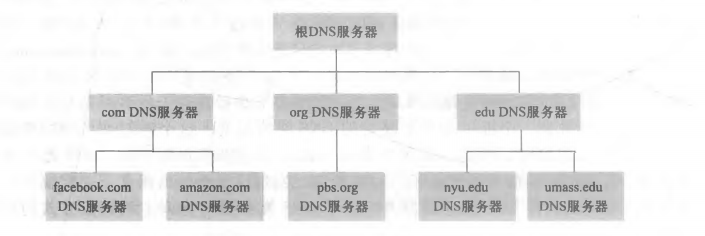
\includegraphics[width=0.6\textwidth]{image/chapter02/DNS层级结构.png}
    \caption{部分DNS服务器的层次结构}
\end{figure}

\begin{itemize}
    \item [1)] 根DNS服务器。有400多个根名字服务器遍及全世界。这些根名字服务器由13个不同的组织管理。根名字服务器提供TLD服务器的IP地址
    \item [2)] 顶级域(DNS)服务器。对于每个顶级域(如com、org、net、edu和gov)和所有家的顶级域(如uk、fr、ca和jp),都有TLD服务器(或服务器集群)。TLD服务器提供了权威DNS服务器的IP地址
    \item [3)] 权威DNS服务器。在因特网上具有公共可访问主机(如Web服务器和邮件服务 器)的每个组织机构必须提供公共可访问的DNS记录,这些记录将这些主机的名字映射为IP地址。
\end{itemize}

    除了上述三种DBS服务器,还有另一类重要的DNS服务器,称为本地DNS服务器(local DNS server)。严格说来,一个本地DNS服务器并不属于该服务器的层次结构,但它对DNS层次结构是至关重要的。

\begin{figure}[!htbp]
    \centering
    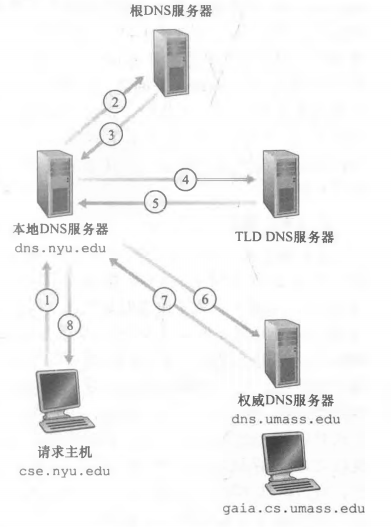
\includegraphics[width=0.6\textwidth]{image/chapter02/各种DNS服务器的交互.png}
    \caption{各种DNS服务器的交互}
\end{figure}

    首先第一步,请求主机将gaia.cs.umass.edu包装成报文发送给本地服务器,本地服务器将该报文转发给根DNS服务器,根DNS服务器注意到.edu信息,并向本地服务器发送负责.edu的TLD的IP地址列表。

    然后,本地服务器通过得到的IP地址列表向TLD服务器发送查询报文,当TLD服务器查询到.umass.edu前缀,并用权威DNS服务器的IP地址进行响应,最终本地服务器直接向权威服务器发送查询报文,权威服务器使用gaia.cs.umass.edu的IP地址进行响应。

    上述所示的例子利用了递归查询(recursive query)和迭代查询(iterative query)。从cse.nyu.edu到dns.nyu.edu发出的查询是递归查询,因为该查询以自己的名义请求dns.nyu.edu来获得该映射。而后继的3个查询是迭代查询,因为所有的回答都是直接返回给dns.nyu.edu。

\subsubsection{DNS缓存}

    实际上,为了改善时延性能并减少在因特网上到处传输的DNS报文数量,DNS广泛使用了缓存技术。DNS缓存的原理非常简单。在一个请求链中,当某DNS服务器接收一个DNS回答(例如,包含某主机名到IP地址的映射)时,它能将映射缓存在本地存储器中。由于主机和主机名与IP地址间的映射并不是永久的,DNS服务器在一段时间后(通常设置为两天)将丢弃缓存的信息

\subsection{DNS记录和报文}

    共同实现DNS分布式数据库的所有DNS服务器存储了资源记录(Resource Record,RR), RR提供了主机名到IP地址的映射。每个DNS回答报文包含了一条或多条资源记录。

    资源记录是一个包含了下列字段的4元组:

$$
    (Name, Value, Type, TTL)
$$

    TTL是该记录的生存时间,它决定了资源记录应当从缓存中删除的时间。在下面给岀的记录例子中,我们忽略掉TTL字段。Name和Value的值取决于Type:

\begin{itemize}
    \item [1)] 如果Type = A,则Name是主机名,Value是该主机名对应的IP地址。因此,一条类型为A的资源记录提供了标准的主机名到IP地址的映射。
    \item [2)] 如果Type = NS,则Name是个域(如foo.com),而Value是个知道如何获得该域中主机IP地址的权威DNS服务器的主机名。这个记录用于沿着查询链来路由DNS查询。
    \item [3)] 如果Type = NAME,则Value是另9名为Name的主机对应的规范主机名。该记录能够向査询的主机提供一个主机名对应的规范主机名
    \item [4)] 如果Type = MX,则Value是个别名为Name的邮件服务器的规范主机名。MX记录允许邮件服务器主机名具有简单的别名。值得注意的是,通过使用MX记录,一个公司的邮件服务器和其他服务器(如它的Web服务器)可以使用相同的别名。为了获得邮件服务器的规范主机名,DNS客户应当请求一条MX记录;而为了获得其他服务器的规范主机名,DNS客户应当请求CNAME记录
\end{itemize}

\subsubsection{DNS报文}

    DNS只有两种报文:DNS查询和回答报文。并且,查询 和回答报文有着相同的格式:

\begin{figure}[!htbp]
    \centering
    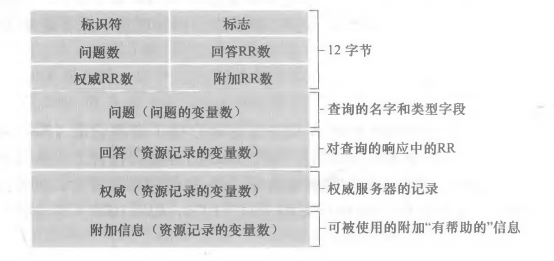
\includegraphics[width=0.6\textwidth]{image/chapter02/DNS报文格式.png}
    \caption{DNS报文格式}
\end{figure}

    对于DNS报文中个字段的语义如下:

\begin{itemize}
    \item [1)] 受不了了,,,以后有精力再看吧。。
\end{itemize}

\section{视频流和内容分发网}

\subsection{因特网视频}

    在流式存储视频应用中,基础的媒体是预先录制的视频,例如电影、电视节目、录制好的体育事件或录制好的用户生成的视频。这些预先录制好的视频放置在服务器上,用户按需向这些服务器发送请求来观看视频。

    从网络的观点看,也许视频最为突出的特征是它的高比特率。压缩的因特网视频的比特率范围通常从用于低质量视频的100kbps,到用于流式高分辨率电影的超过3Mbps,再到用于4K流式展望的超过10Mbps。这能够转换为巨大的流量和存储,特别是对高端视频。例如,单一2Mbps视频在67分钟期间将耗费1GB的存储和流量。到目前为止,对流式视频的最为重要的性能度量是平均端到端吞吐量。为了提供连续不断的布局,网络必须为流式应用提供平均吞吐量,这个流式应用至少与压缩视频的比特率一样大

\subsection{HTTP流和DASH}

    在HTTP流中,视频只是存储在HTTP服务器中作为一个普通的文件,每个文件有一个特定的URL。

    当用户要看该视频时,客户与服务器创建一个TCP连接并发送对该URL的HTTP GET请求。服务器则以底层网络协议和流量条件允许的尽可能快的速率,在一个HTTP响应报文中发送该视频文件。在客户一侧,字节被收集在客户应用缓存中。一旦该缓存中的字节数量超过预先设定的门限,客户应用程序就开始播放,特别是,流式视频应用程序周期性地从客户应用程序缓存中抓取帧,对这些帧解压缩并且在用户屏幕上展现。因此,流式视频应用接收到视频就进行播放,同时缓存该视频后面部分的帧。

    尽管HTTP流在实践中已经得到广泛部署,但它具有严重缺陷,即所有客户接收到相同编码的视频,尽管对不同的客户或者对于相同客户的不同时间而言,客户可用的带宽大小有很大不同。这导致了一种新型基于HTTP的流的研发,它常常被称为经HTTP的动态适应性流(Dynamic Adaptive Streaming over HTTP, DASH)。在DASH中,视频编码为几个不同的版本,其中每个版本具有不同的比特率,对应于不同的质量水平。客户动态地请求来自不同版本且长度为几秒的视频段数据块。

    DASH允许客户使用不同的以太网接入速率流式播放具有不同编码速率的视频。使用DASH后,每个视频版本存储在HTTP服务器中,每个版本都有一个不同的URL。HTTP服务器也有一个告示文件(manifest file),为每个版本提供了一个URL及其比特率。客户首先请求该告示文件并且得知各种各样的版本。然后客户通过在HTTP GET请求报文中对每块指定一个URL和一个字节范围,一次选择一块。在下载块的同时,客户也测量接收带宽并运行一个速率决定算法来选择下次请求的块。

\section{套接字编程:生成网络应用}

\subsubsection{UDP套接字编程}

    现在我们仔细观察使用UDP套接字的两个通信进程之间的交互。在发送进程能够将数据分组推出套接字之门之前,当使用UDP时,必须先将目的地址附在该分组之上。在该分组传过发送方的套接字之后,因特网将使用该目的地址通过因特网为该分组选路到接收进程的套接字。当分组到达接收套接字时,接收进程将通过该套接字取回分组,然后检查分组的内容并采取适当的动作。

    目的主机的IP地址是目的地址的一部分。通过在分组中包括目的地的IP地址,因特网中的路由器将能够通过因特网将分组选路到目的主机。但是因为一台主机可能运行许多网络应用进程,每个进程具有一个或多个套接字,所以在目的主机指定特定的套接字也是必要的。当生成一个套接字时,就为它分配一个称为端口号(port number)的标识符。因此,如你所期待的,分组的目的地址也包括该套接字的端口号。总的来说,发送进程为分组附上目的地址,该目的地址是由目的主机的IP地址和目的地套接字的端口号组成的。此外, 如我们很快将看到的那样,发送方的源地址也是由源主机的IP地址和源套接字的端口号组成,该源地址也要附在分组之上。然而,将源地址附在分组之上通常并不是由UDP应用程序代码所为,而是由底层操作系统自动完成的。

\begin{itemize}
    \item [1)] 客户从其键盘读取一行字符(数据)并将该数据向服务器发送。
    \item [2)] 服务器接收该数据并将这些字符转换为大写。
    \item [3)] 服务器将修改的数据发送给客户。
    \item [4)] 客户接收修改的数据并在其监视器上将该行显示出来
\end{itemize}

\begin{figure}[!htbp]
    \centering
    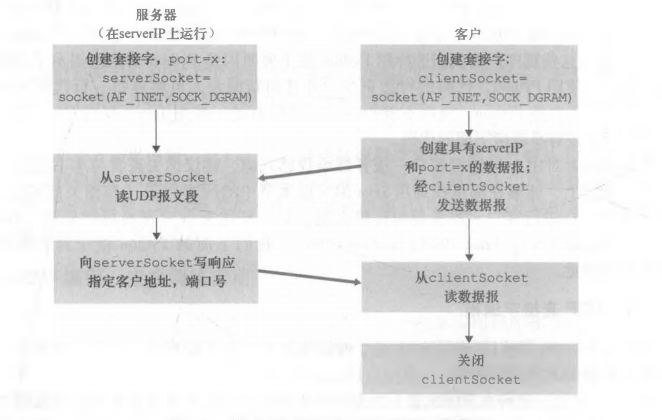
\includegraphics[width=0.6\textwidth]{image/chapter02/UDP服务流程.png}
    \caption{使用UDP的客户-服务器应用}
\end{figure}

\begin{lstlisting}[language=C++, caption={udp client code}]
#include <cstring>
#include <iostream>
#include <netinet/in.h>
#include <string>
#include <sys/socket.h>
#include <arpa/inet.h>

const std::string SERVER_ADDR = "127.0.0.1";
const int PORT = 8081;
const size_t BUFFER_SIZE = 1024;

int main() {
    int sock_fd;
    char buffer[BUFFER_SIZE] = {};
    struct sockaddr_in server_addr;

    if ((sock_fd = socket(AF_INET, SOCK_DGRAM, 0)) < 0) {
        std::cerr << "socket fail" << std::endl;
        exit(-1);
    }

    memset(&server_addr, 0, sizeof server_addr);
    server_addr.sin_family = AF_INET;
    server_addr.sin_addr.s_addr = inet_addr(SERVER_ADDR.c_str());
    server_addr.sin_port = htons(PORT);

    socklen_t server_len = sizeof(sockaddr);
    while (true) {
        std::cout << "[CLIENT]: ";
        gets(buffer);
        sendto(sock_fd, (const char*)buffer, sizeof buffer, 0, (const struct sockaddr*)&server_addr, server_len);

        memset(buffer, 0, BUFFER_SIZE);
        ssize_t len = recvfrom(sock_fd, (char*)buffer, BUFFER_SIZE, 0, (struct sockaddr*)&server_addr, &server_len);
        if (len < 0) {
            std::cerr << "recv fail" << std::endl;
            exit(-1);
        }
        std::cout << "[CLIENT RECV]: "<< buffer << "\n";
    }
    return 0;
}
\end{lstlisting}

\begin{lstlisting}[language=C++, caption={udp server code}]
#include <cstring>
#include <iostream>
#include <arpa/inet.h>
#include <netinet/in.h>
#include <sys/socket.h>
#include <string>

const size_t BUFFER_SIZE = 1024;
const int PORT = 8081;

int main(int, char**){
    int sock_fd;
    sockaddr_in server_addr, client_addr;
    char buffer[BUFFER_SIZE];

    if ((sock_fd = socket(AF_INET, SOCK_DGRAM, 0)) < 0) {
        std::cerr << "socket fail" << std::endl;
        exit(-1);
    }

    memset(&server_addr, 0, sizeof server_addr);
    memset(&client_addr, 0, sizeof client_addr);

    server_addr.sin_family = AF_INET;
    server_addr.sin_addr.s_addr = INADDR_ANY;
    server_addr.sin_port = htons(PORT);

    if (bind(sock_fd, (const sockaddr*)&server_addr, sizeof server_addr) < 00) {
        std::cerr << "bind fail" << std::endl;
        exit(-1);
    }

    socklen_t client_len = sizeof(client_addr);

    while (true) {
        memset(buffer, 0, sizeof buffer);
        ssize_t len = recvfrom(sock_fd, (char*)buffer, BUFFER_SIZE, 0, (sockaddr*)&client_addr, &client_len);
        if (len < 0) {
            exit(-1);
        }
        buffer[len] = '\0';
        std::cout << "[SERVER RECV]: " << buffer << "\n";
        for (char& c : buffer) {
            if (islower(c)) {
                c = toupper(c);
            }
        }
        sendto(sock_fd, (const char*)buffer, sizeof buffer, 0, (const sockaddr*)&client_addr, client_len);
    }
    return 0;
}    
\end{lstlisting}

\subsection{TCP套接字编程}

    与UDP不同,TCP是一个面向连接的协议。这意味着在客户和服务器能够开始互相发送数据之前,它们先要握手和创建一个TCP连接。TCP连接的一端与客户套接字相联系,另一端与服务器套接字相联系。当创建该TCP连接时,我们将其与客户套接字地址(IP地址和端口号)和服务器套接字地址(IP地址和端口号)关联起来。使用创建的TCP连接,当一侧要向另一侧发送数据时,它只需经过其套接字将数据丢进TCP连接。这与UDP不同,UDP服务器在将分组丢进套接字之前必须为其附上一个目的地地址。

\begin{figure}[!htbp]
    \centering
    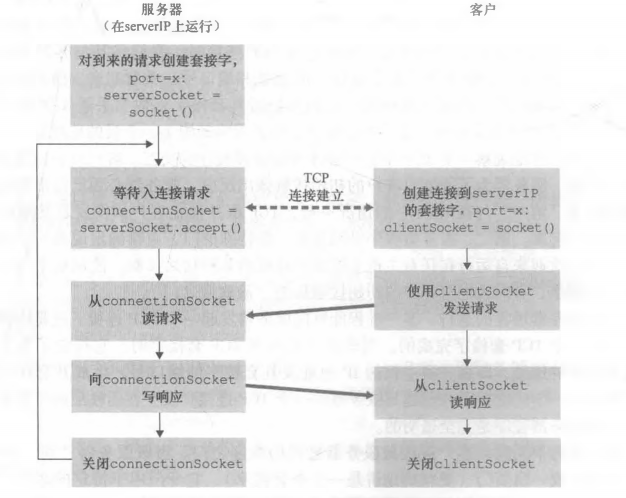
\includegraphics[width=0.6\textwidth]{image/chapter02/TCP服务流程.png}
    \caption{使用TCP的客户-服务器应用}
\end{figure}

\begin{lstlisting}[language=C++, caption={tcp server code}]
#include <cstring>
#include <iostream>
#include <arpa/inet.h>
#include <netinet/in.h>
#include <sys/socket.h>
#include <string>
#include <unistd.h>

const size_t BUFFER_SIZE = 1024;
const int PORT = 8081;

int main(int, char**){
    int sock_fd, clinet_sock;
    sockaddr_in server_addr, client_addr;
    char buffer[BUFFER_SIZE];

    if ((sock_fd = socket(AF_INET, SOCK_STREAM, 0)) < 0) {
        std::cerr << "socket fail" << std::endl;
        exit(-1);
    }

    memset(&server_addr, 0, sizeof server_addr);
    memset(&client_addr, 0, sizeof client_addr);

    server_addr.sin_family = AF_INET;
    server_addr.sin_addr.s_addr = INADDR_ANY;
    server_addr.sin_port = htons(PORT);

    if (bind(sock_fd, (const sockaddr*)&server_addr, sizeof server_addr) < 0) {
        std::cerr << "bind fail" << std::endl;
        exit(-1);
    }

    if (listen(sock_fd, 5) < 0) {
        std::cerr << "listen fail" << std::endl;
        exit(-1);
    }

    socklen_t client_len = sizeof(client_addr);

    clinet_sock = accept(sock_fd, (sockaddr*)&client_addr, &client_len);

    while (true) {
        memset(buffer, 0, sizeof buffer);
        ssize_t len = read(clinet_sock, buffer, BUFFER_SIZE);
        if (len < 0) {
            exit(-1);
        }
        buffer[len] = '\0';
        std::cout << "[SERVER RECV]: " << buffer << "\n";
        for (char& c : buffer) {
            if (islower(c)) {
                c = toupper(c);
            }
        }
        send(clinet_sock, buffer, sizeof buffer, 0);
    }
    return 0;
}
\end{lstlisting}

\begin{lstlisting}[language=C++, caption={tcp client code}]
#include <cstring>
#include <iostream>
#include <netinet/in.h>
#include <string>
#include <sys/socket.h>
#include <arpa/inet.h>
#include <unistd.h>

const std::string SERVER_ADDR = "127.0.0.1";
const int PORT = 8081;
const size_t BUFFER_SIZE = 1024;

int main() {
    int sock_fd;
    char buffer[BUFFER_SIZE] = {};
    struct sockaddr_in server_addr;

    if ((sock_fd = socket(AF_INET, SOCK_STREAM, 0)) < 0) {
        std::cerr << "socket fail" << std::endl;
        exit(-1);
    }

    memset(&server_addr, 0, sizeof server_addr);
    server_addr.sin_family = AF_INET;
    server_addr.sin_addr.s_addr = inet_addr(SERVER_ADDR.c_str());
    server_addr.sin_port = htons(PORT);

    if (connect(sock_fd, (sockaddr*)&server_addr, sizeof server_addr) < 0) {
        std::cerr << "connect fail" << std::endl;
        exit(-1);
    }

    socklen_t server_len = sizeof(sockaddr);
    while (true) {
        std::cout << "[CLIENT]: ";
        gets(buffer);
        send(sock_fd, buffer, sizeof buffer, 0);

        memset(buffer, 0, BUFFER_SIZE);
        ssize_t len = read(sock_fd, buffer, BUFFER_SIZE);
        if (len < 0) {
            std::cerr << "recv fail" << std::endl;
            exit(-1);
        }
        std::cout << "[CLIENT RECV]: "<< buffer << "\n";
    }
    return 0;
}
\end{lstlisting}

\section{课后习题}

    有时间,再做!下次一定!